\documentclass[letterpaper,12pt,fleqn]{article}
\usepackage{matharticle}
\usepackage{siunitx}
\pagestyle{empty}

\newcommand{\Rel}{\mathcal{R}}

\begin{document}

\section*{Relations}

\begin{itemize}[left=0in]

\item Physical phenomena are characterized by certain quantities and the how those quantities are \emph{related} to
  each other.

\item Each quantity is associated with a set that contains the possible values for that quantity.  In precalculus
  and calculus these sets are almost always subsets of \(\R\).

\item Each quantity is assigned a variable that can assume elements of the associated set.

\item To show that \(a\in A\) \emph{is related to} \(b\in B\), use the ordered pair \((a,b)\).  This answers the
  question, ``What is the value of the \(B\) quantity given the value of the \(A\) quantity.''  In fact, \(a\) is
  acting like an \emph{input} value and \(b\) is acting like an \emph{output} value.

\item If each possible \(a\in A\) is associated with exactly one \(b\in B\) then the relation is
  \emph{well-defined}.  Otherwise, the relation is \emph{not well-defined}.
\end{itemize}

\begin{example}[A Chemical Reaction]
  Quantities:

  \begin{itemize}
  \item Mass of a reactant: \(r\in[0,\infty]\)
  \item Mass of a product: \(p\in[0,\infty]\)
  \item Heat energy absorbed (endothermic) or emitted (exothermic): \(h\in\R\)
  \item Time: \(t\in[0,\infty)\)
  \end{itemize}

  Relations:

  \begin{itemize}
  \item How much product has been produced by a given time?: \((t,p)\), well-defined.
  \item How much time has passed when a certain amount of product has been produced?: \((p,t)\), well-defined.
  \item How much energy has been released when a certain amount of a reactant has been consumed?: \((r,h)\),
    well-defined.
  \end{itemize}

  \begin{center}
    \begin{tikzpicture}
      \draw [help lines,->] (0,0) -- (5,0) node [right] {\(t\)};
      \draw [help lines,->] (0,0) -- (0,3) node [above] {\(p\)};
      \draw [domain=0:5,blue] plot ({\x},{2*(1-exp(-\x)});
      \node [closed point,red] (X) at (2,{2*(1-exp(-2)}) {};
      \draw [dashed] (X) -- (2,0) node [below] {\(t\)};
      \draw [dashed] (X) -- (0,{2*(1-exp(-2)}) node [left] {\(p\)};
    \end{tikzpicture}
  \end{center}
\end{example}

\newpage

\begin{example}[The Flight of an Aircraft]
  Quantities:

  \begin{itemize}
  \item Distance traveled: \(d\in[0,\infty)\)
  \item Altitude: \(a\in[0,\infty)\)
  \item Airspeed: \(s\in[0,\infty)\)
  \item Time: \(t\in[0,\infty)\)
  \end{itemize}

  Relations:

  \begin{itemize}
  \item What is the aircraft's altitude at a given time?: (t,a), well-defined.
  \item At what times is the aircraft at a particular altitude?: (a,t), not well-defined.
  \end{itemize}

  \begin{center}
    \begin{tikzpicture}
      \draw [help lines,->] (0,0) -- (10,0) node [right] {\(t\)};
      \draw [help lines,->] (0,0) -- (0,3) node [above] {\(p\)};
      \draw [blue,rounded corners=0.5cm] (0,0) -- (1,0) -- (2,2) -- (8,2) -- (9,0) -- (10,0);
      \node [closed point,red] (X1) at (3,2) {};
      \node [closed point,red] (X2) at (5,2) {};
      \node [closed point,red] (X3) at (7,2) {};
      \draw [dashed] (X1) -- (3,0) node [below] {\(t_1\)};
      \draw [dashed] (X2) -- (5,0) node [below] {\(t_2\)};
      \draw [dashed] (X3) -- (7,0) node [below] {\(t_3\)};
      \draw [dashed] (X3) -- (0,2) node [left] {\(a\)};
    \end{tikzpicture}
  \end{center}
\end{example}

\begin{definition}[Relation]
  A relation \(\Rel\) between a set \(A\) and a set \(B\) is set that is a subset of \(A\times B\):
  \[\Rel\subseteq A\times B=\setb{(a,b)}{a\in A\ \text{and}\ b\in B}\]
\end{definition}

In precalculus and calculus, relations are almost always subsets of \(\R\times\R=\R^2\), which is also known as
the Cartesian plane.

\begin{example}
  There is no limitation on which ordered pairs are included in a relation.  In fact, elements of the relation can
  be selected arbitrarily.  Let \(\Rel\subset\R^2\) where:
  \[\Rel=\set{(0,1), (0,3), (-1,2), (\pi,3), (\sqrt{2},-1),(-3,-3),(3,-3)}\]
  Note that \(\Rel\) is a set of discrete elements and that the values from the two sets can be reused without
  limitations.

  \begin{center}
    \begin{tikzpicture}
      \draw [very thick] (-4,0) -- (4,0);
      \draw [very thick] (0,-4) -- (0,4);
      \draw [very thin,lightgray] (-4,-4) grid (4,4);
      \node [closed point,red] (X1) at (0,1) {} node at (X1) [right] {\((0,1)\)};
      \node [closed point,red] (X2) at (0,3) {} node at (X2) [right] {\((0,3)\)};
      \node [closed point,red] (X3) at (-1,2) {} node at (X3) [left] {\((-1,2)\)};;
      \node [closed point,red] (X4) at ({pi},3) {} node at (X4) [above] {\((\pi,3)\)};
      \node [closed point,red] (X5) at ({sqrt(2)},-1) {} node at (X5) [right] {\((\sqrt{2},-1)\)};
      \node [closed point,red] (X6) at (-3,-3) {} node at (X6) [above] {\((-3,-3)\)};
      \node [closed point,red] (X7) at (3,-3) {} node at (X7) [above] {\((3,-3)\)};
    \end{tikzpicture}
  \end{center}
\end{example}

\begin{example}
  Relations are normally constrained by physical phenomena and can result from measurements taken during an
  experiment or from well-known formulas that \emph{model} the phenomena.  Consider an object thrown into the air
  with a speed of \SI{64}{ft/s}.  Gravity slows and eventually stops the object at a maximum height of \SI{64}{ft}
  and then the object falls back to earth:
  \[\R=\setb{(t,h)}{h=64t-16t^2}\]
  Note that this is a continuous phenomenon and so the relation is an infinite set and thus cannot be specified by
  roster.

  \begin{center}
    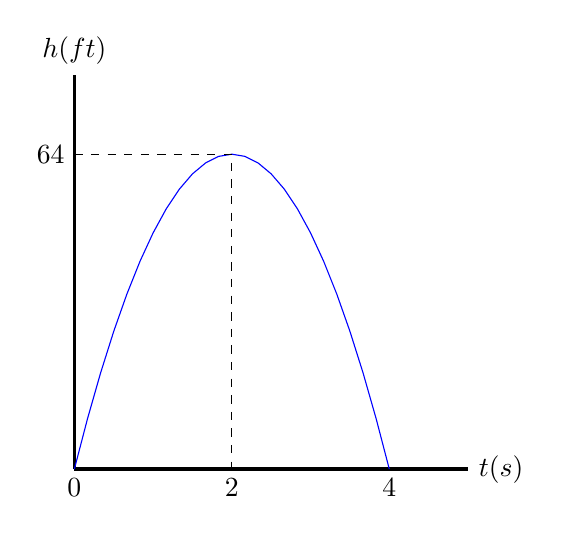
\begin{tikzpicture}
      \draw [very thick] (0,0) -- (5,0) node [right] {\(t(s)\)};
      \draw [very thick] (0,0) -- (0,5) node [above] {\(h(ft)\)};
      \draw [domain=0:4,blue] plot ({\x},{4*\x-\x^2});
      \node [below] at (0,0) {\(0\)};
      \node [below] at (2,0) {\(2\)};
      \node [below] at (4,0) {\(4\)};
      \node [left] at (0,4) {\(64\)};
      \draw [dashed] (0,4) -- (2,4) -- (2,0);
    \end{tikzpicture}
  \end{center}
\end{example}

\end{document}
